\chapter{Planung} \label{chpt:planung}

Bevor mit der Durchführung eines Projekts angefangen werden kann, sollte mithilfe einer Projektdefinition das Projekt geplant werden. Dieses Kapitel beschreibt die Aspekte welche in der Projektdefinition für das Projekt festgelegt wurden. Unter anderem werden die Rahmenbedingungen, der Umfang so wie die Risikobehandlung erläutert.

\section{Projektdefinition}\label{sec:projektdef}
In der Projektdefinition werden das Ziel, eine vereinfachte Strategie zur Erreichung des Ziels und der Bearbeitungszeitraum festgelegt.\\
Das Ziel ergibt sich in  diesem Projekt aus der in \autoref{sec:Aufgabenstellung} genannten Aufgabenstellung und lautet: \glqq Entwicklung einer Android-App mit Checklisten Funktion\grqq.
Die Strategie wurde sehr simpel gehalten und ist: \glqq Projektumfang planen und App entwickeln\grqq. Diese vereinfachte Beschreibung der Strategie ist darauf zurückzuführen, dass es sich um ein Ein-Mann Projekt handelt und eine weitere Ausführung zur eventuellen Aufgabenteilung nicht als nötig erachtet wurde.
Der Projektstart ist die offizielle Start der Studienarbeit der \ac{DHBW} am 01.10.2020. Das Ende des Projektes spiegelt der Abgabetermin der Studienarbeit am 17.05.2021 wieder

\section{Rahmenbedingungen}\label{sec:rehamen}
Mithilfe von Rahmenbedingungen werden die Grenzen des Projekts erstmals festgelegt. Gleichermaßen legen die Rahmenbedingungen grundlegende Entscheidungen fest, welche für die Durchführung des Projekts relevant sind. Die Rahmenbedingungen, welche in der Projektdefinition festgelegt wurden sind:

\begin{itemize}
	\item Android Studio wird als \ac{IDE} verwendet
	\item Es wird ausschließlich eine Android und keine iOS-App entwickelt
	\item Das Projekt wird in der Studienarbeit beschrieben und von dem Betreuer Dr. Christian Bomhardt bewertet
\end{itemize}

Diese Rahmenbedingungen wurden aus bestimmten Gründen festgelegt, welche im folgenden erläutert werden.
Der zweite Punkt grenzt die Entwicklung auf eines der zwei breit vertretenen Betriebssystemen für mobile Endgeräte ein. Hierbei wurde sich auf das Betriebssystem Android von Google festgelegt. Es wurde sich aus zwei Gründen bewusst gegen iOS entschieden. Der erste ist die Entwicklungsumgebung. Zur Entwicklung wird das von Apple entwickelte Programm Xcode benötigt. Um dieses zu herunterzuladen wird eine Apple-ID vorausgesetzt welche sich nun fließend mit dem zweiten Problempunkt in Verbindung bringen lässt. Die Apple-ID bezieht sich auf den eigenen Apple-Account. Jeder der ein Apple Produkt besitzt hat in der Regel einen solchen Account. Da für dieses Projekt kein Budget zur Verfügung gestellt wird und weder ein Apple-Rechner noch mobile Endgeräte vorhanden sind kann weder eine App mit dem bereits genannten Programm Xcode entwickelt noch die App auf einen physischen Gerät getestet werden. Im Gegensatz zu iOS und Apple Produkten sind mehrere Android Geräte vorhanden welche zum testen unter realen Bedingungen genutzt werden können.\footcite{chipIPhone.2019}\footcite{Xcode.2021} \\
Mit der Erläuterung des zweiten Punktes wird auch der erste Punkt deutlicher. Bei Android Studio handelt es sich um die von Android zur Verfügung gestellte Entwicklungsumgebung. Da Android als Grundlegendes Betriebssystem für die App festgelegt wurde ist Android Studio die logische Wahl. Zudem ist Android Studio frei verfügbar und lässt sich auf Windows-Rechnern installieren. Als Bonus wir es sogar mit der JetBrains Toolbox ausgeliefert, was die Installation und Aktualisierung des Programm weiter vereinfacht.\footcite{AndroidStudio.2021} \\
Der dritte Punkt bezieht sich auf die Bewertung und den Abschluss des Projekts. Die Studienarbeit dient als Dokumentation und Projektabschluss sowie als Grundlage zur Benotung des Projekts im Rahmen der Studienarbeit an der \ac{DHBW} Karlsruhe. Bei der Studienarbeit handelt es sich um dieses Dokument. Die Benotung wird von dem Betreuer der Studienarbeit Dr. Christian Bomhardt vorgenommen.\\
Da die Rahmenbedingung jetzt ausführlich erläutert wurden wird im nächsten Abschnitt (\ref{sec:umfang}) der Umfang der App ausgeführt.

\section{Umfang}\label{sec:umfang}

Der Umfang legt die innerhalb des Rahmens zu erledigenden Aufgaben fest. Er ist sozusagen der Soll-Betrag, welcher zur Erreichung des Ziels benötigt wird. Im Zuge der App Entwicklung wurden hier die Anwendungsfälle festgelegt, welche in der App ausführbar sein müssen. Diese Anwendungsfälle sind:

\begin{itemize}
	\item Erstellen einer Checkliste
	\item Bearbeiten einer Checkliste
	\item Löschen einer Checkliste
	\item Erstellen einer Aufgabe
	\item Bearbeiten einer Aufgabe
	\item Löschen einer Aufgabe
	\item Abhacken einer Aufgabe
	\item Hacken von einer Aufgabe entfernen
	\item Hacken von allen Aufgaben einer Checkliste entfernen
\end{itemize}

Die hier genannten Anwendungsfälle orientieren sich an der in \autoref{sec:Aufgabenstellung} festgelegten Aufgabenstellung.
Es soll dem Benutzer der App möglich sein in der Anwendung neue Checklisten anzulegen, um so für jede dem Nutzer nötige Situation eine Checkliste zur Verfügung zu haben. Da es sich um eine anpassbare Checkliste handeln soll, muss der Benutzer die Möglichkeit haben die Checkliste zu Bearbeiten. Im selben Zusammenhang sollte es dem Benutzer auch möglich sein nicht mehr benötigte Checklisten wieder zu löschen. Um die Checkliste nutzbar zu machen soll der Benutzer in der Lage sein Aufgaben in einer Checkliste zu erstellen. Im Sinne der Nutzererfahrung und Anpassbarkeit der Checkliste soll es ebenfalls möglich sein erstellte Aufgaben zu bearbeiten und auch wieder zu löschen. Die letzten drei Anwendungsfälle sind der Kern der Anwendung. Es muss dem Nutzer ermöglicht werden eine Aufgabe als erledigt zu markieren und diese Markierung auch wieder zu entfernen. In der Liste der Anwendungsfälle wird das Markieren beispielshaft als abhacken und entfernen des Hacken betitelt. Diese acht Anwendungsfälle stellen die Grundlage dar, welche die App erfüllen muss um als Nutzbar angesehen zu werden. Der neunte Punkt stellt eine zusätzliche Funktion dar, die dem Benutzer die Handhabung erleichtern soll. Bei diesem Anwendungsfall sollen die \glqq Hacken\grqq{} aller Aufgaben innerhalb einer Checkliste entfernt werden. Dadurch muss der Benutzer nicht selbst alle Hacken entfernen, wenn er die Checkliste wieder benutzen will und spart dadurch Zeit und Aufwand. Zusätzlich soll es bei dem Benutzer zu einer besseren Benutzererfahrung führen.\\
Nachdem die Anwendungsfälle geklärt sind wird nun weiter auf die Checkliste und Aufgabe an sich eingegangen. Diese stellen als Klasse die Modelle dieser Objekte dar. \autoref{fig:KlassenDiagramm} zeigt den Aufbau der Checkliste und der Aufgabe anhand eines Klassendiagramm. Beide Klassen haben einen Titel und eine Beschreibung als String Attribut. Die Checkliste hält zusätzlich eine Liste von Aufgaben, einen sogenannten Array von Aufgaben. Die Aufgabe auf der anderen Seite hat als zusätzliches Attribut Abgehackt als Boolean. Die Checkliste hat neben den get- und set-Methoden jeweils eine Methode zum hinzufügen und entfernen von Aufgaben in das Aufgaben-Array Attribut. Die Aufgaben Klasse hat nur die get- und set-Methoden. 

\begin{figure}[h]
	\centering
	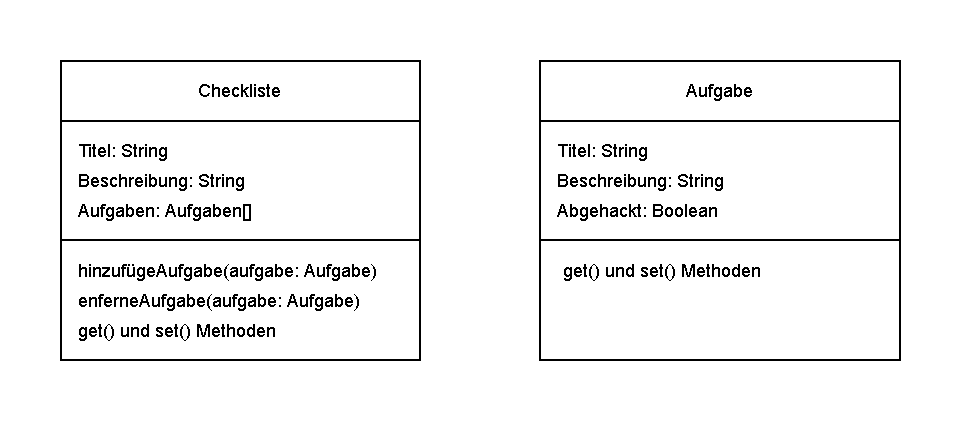
\includegraphics{Bilder/KlassenDiagramm.pdf} 
	\caption{Klassen-Diagramm zu den Grundlegenden Klassen Checkliste und Aufgabe}
	\label{fig:KlassenDiagramm}
\end{figure}

Nach dem Entwickeln und Implementieren der Anwendungsfälle sollen diese getestet werden. Hierfür sind im Umfang der Projektdefinition Espresso-\ac{UI} Test vorgesehen. Mithilfe dieser Test können die Abläufe der Anwendungsfälle simuliert auf dem Emulator von Android Studio durchgeführt werden und so die Funktionalität gewährleistet werden. In der ursprünglichen Projektdefinition ist definiert, dass mindestens 80\% der Anwendungsfälle mithilfe von Espresso Tests getestet werden sollen.\\
Als letztes legt die Definition des Umfang fest, dass eine Studienarbeit mit dem von der \ac{DHBW} Karlsruhe vorgegebenen Umfang von 40-60 Seiten geschrieben werden muss.\\

Nach Rücksprache mit dem Betreuer sind Ideen für eine Erweiterung des Umfang aufgetreten. Dabei handelt es sich um folgende Anwendungsfälle beziehungsweise Erweiterungen:

\begin{itemize}
	\item Push-Benachrichtigungen bei dem verlassen eines für die Checkliste festgelegten Ort.
	\item Zeitstempel an den Aufgaben
	\item Historie
\end{itemize}

Der erste Punkt ist ein weiterer Anwendungsfall der verhindern soll, dass Nutzer vergessen die App und somit die Checkliste zu öffnen. Als Anhaltspunkt wurde die GeoFencing \ac{API} genannt. Der zweite Punkt handelt von der Erweiterung der Aufgaben Klasse um ein Zeitstempel Attribut. Dieser soll den Fall vorbeugen, dass die Hacken vom vorherigen Tag noch vorhanden sind und der Nutzer so nicht weiß ob er diese Aufgaben am aktuellen Tag bereits erledigt hat. Der dritte Punkt spiegel eine Erweiterung des Zeitstempel als eigenen Anwendungsfall wieder. Hierbei soll die komplette Checkliste für einen festgelegten Zeitraum in einer Historie gespeichert werden. Dies soll dem Nutzer ermöglichen den Zustand der Aufgaben von vorherigen Tagen noch einmal einsehen zu können und sich so versichern zu können die Aufgabe erledigt zu haben.

\section{Risikobehandlung}\label{sec:risiko}

Zum Schluss des Planungskapitel und somit der ursprünglichen Projektdefinition wird das Thema Risikobehandlung behandelt.
Die Risikobehandlung dient dem einschätzen und eingrenzen von Risiken. Dabei werden mögliche Risiken erfasst und beschrieben. Dazu zählen das Risiko, eine Beschreibung zu dem Risiko, eine geschätzte Wahrscheinlichkeit zu der das Risiko eintritt und eine Alternative mit welcher im Falle des Auftretens die Auswirkungen aufgefangen oder abgemildert werden sollen. In \autoref{tabelle:Risko} wird die Risikobehandlung aus der Projektdefinition dargestellt.
\begin{table}[h]
	\centering
	\caption{Risikobehandlung}
	\begin{tabularx}{\textwidth}{|X|X|>{\centering\arraybackslash}X|X|}
		\toprule
		Risiko  & Beschreibung & Wahrscheinlichkeit & Alternative\\ \midrule 
		Verspäteter Projektstart  & Die Bearbeitung des Studienarbeitsprojekt wird verspätet angefangen & 80\%  & Verlorene Zeit wird zu einem späteren Zeitpunkt durch längere Arbeitstage und Wochenendschichten aufgeholt \\ \midrule
		Umfang nicht eingehalten & Aufgrund von Zeit oder Wissensmangel nicht alle Anwendungsfälle in der App implementiert & 20\% & Leistungsumfang im Bereich des möglichen verringern \\ \midrule
		Krankheit & Verminderter Fortschritt aufgrund von Krankheit & 20\% & Krankheit so gut wie möglich vermeiden, verlorene Zeit später aufholen \\ \midrule
		Vernachlässigte Dokumentation & Nicht alle Ideen und konkret geplante Umsetzungen vor der Implementierung dokumentiert & 50\% & Wenn möglich Dokumentation nachholen (Bsp. Diagramme) \\
		\bottomrule
	\end{tabularx}
	\label{tabelle:Risko}
\end{table}

Wie in \autoref{tabelle:Risko} zu sehen ist hält sich die Anzahl an Risiken in grenzen. Dies ist darauf zurückzuführen das nur eine Person und kein Team an dem Projekt arbeitet. Dadurch können \zB keine Kommunikationsprobleme auftreten. Ausfälle einzelner Personen und somit Nichterfüllung derer Aufgabenteile reflektieren hier das ganze Projekt und könnten somit alle mit den vier genannten Risiken abgedeckt werden.\\
Da es sich bei den in der Tabelle aufgeführten Risiken um die aus der Projektdefinition handelt werden eventuelle Eintritte und Erweiterungen im folgenden erläutert.\\
Das Risiko des verspäteten Projektstart ist, wie anfangs korrekt eingeschätzt wurde, eingetreten. Damit hat sich die Eintrittwahrscheinlichkeit von 80\% bestätigt. Das Eintreten des Risiko ist auf eine schlechte Angewohnheit des Verantwortlichen zurückzuführen. Die Alternative zu diesem Risiko befindet sich in Ausübung und wird mit Ende der Ausarbeitung der Studienarbeit als erfolgreich angesehen.\\
Das zweit genannte Risiko konnte nach Projektdefinitionsstand erfolgreich verhindert werden. Das Risiko wird jedoch hiermit um \glqq Erweiterungsumfang nicht eingehalten\grqq{} erweitert, da nach Rücksprache mit dem Betreuer Ideen für weitere Anwendungsfälle aufgetreten sind. Die Wahrscheinlichkeit für dieses angepasste Risiko wird somit im Nachhinein auf 60\% angehoben. Die Alternative für den Eintritt des Risiko wird beibehalten und vermutlich Anwendung für den Großteil der Ideen finden.\\
Die vernachlässigte Dokumentation ist ebenfalls in kleinerem Rahmen eingetreten. Die Studienarbeit selbst gilt als Hauptaspekt der Dokumentation und wird sicher fertiggestellt. Der eingetretene Bereich bezieht sich auf das Erstellen von \ac{UML}-Diagrammen. Hier tritt ebenfalls die Alternative in Kraft und die Diagramme werden nach Bedarf erstellt.\\
Das Risiko Krankheit konnte zu 100\% vermieden werden.\\
In Folge des \autoref{chpt:durchfuerung} \nameref{chpt:durchfuerung} werden unerwartete Probleme aufgeführt, welche Aufgrund des unerwarteten Eintritts keine Berücksichtigung in der Risikobehandlung gefunden haben. Diese werden im \autoref{sec:problem} \nameref{sec:problem} behandelt.\\

Mit Abschluss der Risikobehandlung gilt das \autoref{chpt:planung} \nameref{chpt:planung} als abgeschlossen. In diesem Kapitel wurden die Projektdefinition welche zu Beginn des Projekts stattgefunden hat behandelt. Es wurde die konkrete Projektdefinition ausgeführt und mithilfe der Rahmenbedingungen und des Umfang eingegrenzt und konkretisiert. Als Abschluss wurde auf die Risikobehandlung eingegangen und eventuelle Eintritte und Änderungen erläutert.